%\documentclass[conference]{IEEEtran}
\documentclass[twocolumn]{article}
\usepackage{lipsum}
%IEEEoverridecommandlockouts
% The preceding line is only needed to identify funding in the first footnote. If that is unneeded, please comment it out.
\usepackage{cite}
\usepackage[utf8]{inputenc}
\usepackage[margin=1.0in]{geometry}
\usepackage{amsmath,amssymb,amsfonts}
\usepackage{algorithmic}
\usepackage{graphicx}
\usepackage{apacite}
\usepackage{natbib}
\usepackage{textcomp}
\usepackage{multirow}
\usepackage{multicol}
\usepackage{float}
\usepackage{xcolor}
%\usepackage{fullpage}
\usepackage{times}
\usepackage{enumitem}
\usepackage{amsmath}
\usepackage{stackengine}
\usepackage{algorithm}
\usepackage{algorithmic}
\usepackage{fancyhdr,graphicx,amsmath,amssymb}
\usepackage[ruled,vlined]{algorithm2e}
\usepackage{caption}
\usepackage{hyperref}
\hypersetup{
    colorlinks=true,
    linkcolor=black,
    citecolor=blue,
    filecolor=magenta,      
    urlcolor=blue
    }
\captionsetup[table]{skip=5pt}
\include{pythonlisting}
\def\BibTeX{{\rm B\kern-.05em{\sc i\kern-.025em b}\kern-.08em
    T\kern-.1667em\lower.7ex\hbox{E}\kern-.125emX}}

\begin{document}

\title{CS 534 Group 1: Utilizing Genetic Algorithms to Develop an Efficient Traffic Light Autonomous Agent}
\author{Keith Chester \thanks{e-mail: kchester@wpi.edu}, Bob DeMont \thanks{e-mail: rldemont@wpi.edu}, Jonathan Landay \thanks{e-mail: jrlanday@wpi.edu}, Jesse Morzel \thanks{e-mail: jemorzel@wpi.edu}}
\date{July 21, 2022}   % The report due date

\maketitle

\begin{abstract}

We propose a novel agent for controlling a collection of traffic lights across a complex city grid of intersecting streets. This agent will be fed approximate traffic counts of vehicles at each light and their directions as input. From this the agent must coordinate light timings. We shall be utilizing an evolutionary algorithm to train an agent against a fitness function that minimizes the delayed time of vehicles moving to their destination. An efficient agent should maintain a low total waiting time for vehicles trying to move through the city.

\end{abstract}

\subsection*{Keywords}
traffic light control, neural network, evolutionary algorithm


\section{Introduction}

\subsection{Motivational Background}

We have chosen this domain as it has a high reach and impact upon the lives of people, ourselves included. The average American drives 25 miles, or one hour behind the wheel, each day. In 2019 the average American had 99 hours of time spent in traffic a year (\cite{INRIX}). While traffic lights are not the sole contributor to congestion, they can be wielded in a precise manner to combat congestion - or bluntly and add to this congestion (see Figure ~\ref{fig:traffic_lights}). Research into the root cause of congestion in urban areas has found that delays caused by intersections can make up between 12-55 \% of total travel time (\cite{Jones}). A reduction in time spent in traffic will result in increased productivity across an entire city, reduced pollution, reduced fuel consumption and allow us some much needed spare time for far more relaxing enterprises.

Traffic lights are generally controlled via cycle time and phase duration.  Cycle time is the time to complete a complete cycle from, for example, start of green on an east-west road through all changes to the start of green east-west.  Each of the light changes is a phase.  Phase duration can vary as we've noted, by schedule or by actuation, and a State constitutes the current condition of the light in each direction.

Currently many traffic light controlled intersections are controlled with a static schedule of timed durations based on the time of day and a database of expected traffic densities, or traffic actuated based on induction coil inputs or a combination of these two methods. Generally any coordination among lights is accomplished based on a master clock concept rather than communication among devices. Because of the uncertainty of traffic arrivals, it is difficult to optimize either scheduled or actuated signals.  
The US Department of Transportation (DOT) publishes guidelines for traffic light phase (green, yellow, and red) as a function of total cycle length and traffic flow based on an 85th to 95th percentile probability of queue clearance. For example, for a traffic light with a total cycle time of 60 seconds and traffic flow of 100 vehicles per hour per lane, the US DOT guidelines recommend a maximum green phase of 15 seconds (\cite{USDOT}). However, this approach is based on average traffic data collected nationwide and by design will only clear the queue at a traffic light 85-95\% of the time. For improved performance, more intelligent techniques are required which can learn and react to real-time traffic conditions.

\begin{figure}[htp]
    \centering
    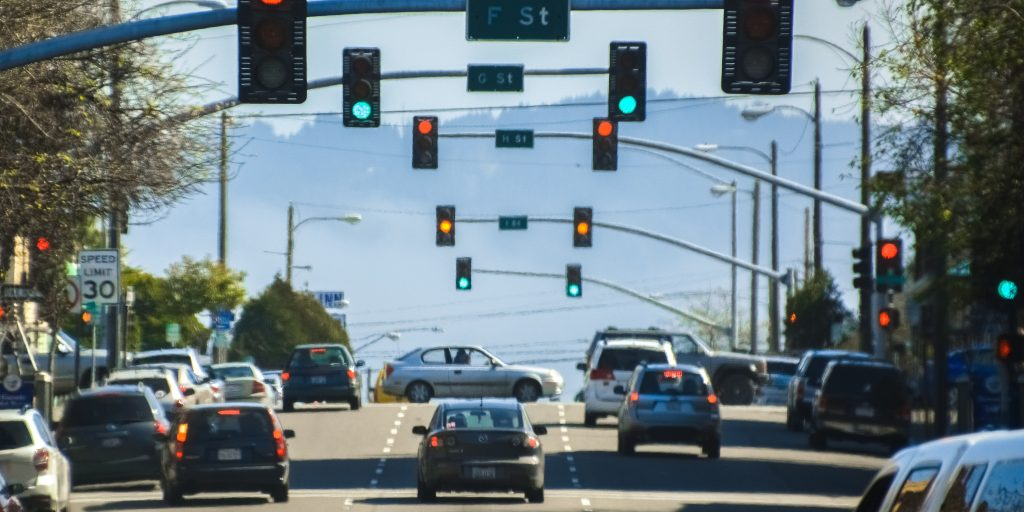
\includegraphics[width=8cm]{figures/traffic_light_network.jpg}
    \caption{Network of Traffic Lights}
    \label{fig:traffic_lights}
\end{figure}

Immediate benefits of a successful outcome to this paper could be improved traffic flow, reduced emissions, reduced waiting time, and lower personal frustration for drivers in traffic light controlled environments around the world.  
\subsection{State of the Art}

Much recent research is exploring coordination through IOT technologies for optimum efficiencies. In most implementations, the two implementations of choice have been genetic algorithms, as seen in \cite{Turky}, \cite{Gora},  \cite{Nwiabu},  \cite{Sofronova}, \cite{Semet}, \cite{Mao},  \cite{Tan}, and  \cite{Fujdiak}, as well as ant colony optimization (ACO) algorithms , as seen in \cite{Rida}, \cite{Dang-Nhac}, and \cite{Nguyen}.

The genetic algorithms provide simple-to-implement solutions that are easy to understand, however this approach suffers in complicated domains where many factors are accounted for with space and time complexity. The genetic algorithms also suffer from early convergence in situations, leading to sub-optimal solutions. The ACO implementations are fairly novel solutions to the problem, however it has not yet been established as converging quickly to an optimal solution, and much more occupies the space of a valid solution, but with room to be improved in both understandability, convergence speed, as well as in some cases the solution cost as well.

\subsection{Novel Approach}

Our novel approach is to consider an evolutionary algorithm to create a singular agent that can control a grouping of traffic lights. This single agent will be fed the cars within a given range at each traffic light and their directions as inputs. This would be accomplished in practice via car detecting cameras and additional sensors at each light. The agent will then calculate appropriate timings to maintain different light patterns, and maintain this as the traffic flows throughout the city. We suspect that a singular agent attempting to coordinate multiple lights across a large area instead of a series of individual agents should result in net less time spent in traffic for the greater population, as compared to a set of individual traffic light agents acting independently. We also expect a decrease in traffic time versus human set schedules, which do not react to dynamic changes in traffic patterns.

We will build a simulation of a city grid with multiple traffic lights and traffic in order to train and evaluate our agent. Our vehicles will be modeled as simplistic agents that will follow traffic rules and move between set destinations. We will record the time each vehicle takes to reach its destination and compare it to the estimated time it would take if it did not encounter any traffic (i.e. an unrealistic ideal travel time). This difference will act as our fitness function for the agent. Through training and evolutionary mating, mutation, and culling we shall create an agent that minimizes this metric.
For comparison of results, we will also have a random agent - setting traffic times to random intervals - and a preset schedule agent, that will have a static schedule for all traffic light times.

\subsection{Outline}

We review related research into applications of AI to traffic light control in section 2. In section 3, we detail the methodology of our genetic algorithm agent as applied to traffic light control, including details about the simulation environment, algorithm design and implementation, and agent training. Experimental results are discussed in section 4 and preliminary conclusions are discussed in section 5.  Section 6 details suggestions for future work and section 7 provides a link to the github repository containing the source code for the project. Finally, we conclude with a list of references cited in this work.


\section{Related Work}
Recent related research generally utilizes algorithms which fall into 2 categories, genetic algorithms and ant colony optimization algorithms.
The first group of methods primarily utilize genetic algorithms in order to induce the learning to optimize the traffic systems.  These algorithms can be found utilized in \cite{Turky}, \cite{Gora}, \cite{Nwiabu}, \cite{Sofronova}, \cite{Semet}, \cite{Mao}, \cite{Tan}, and \cite{Fujdiak}. These algorithms work by generating a set of chromosomes attributed to the independent variables of the problem, such as the number of vehicles per unit time to pass through the direction of the intersection, with which the dependent variable can be simulated. In these situations, the different chromosomes are mutated and reproduce based off an evaluation of fitness, which guides mutation to find an optimal chromosome solution. However, there are limitations to this algorithm. One of which is that a significant increase in number of chromosomes has a very significant impact on the speed and space complexity of the algorithm, leading to much worse performance with many chromosomes. Another limitation is that there are many parameters, such as mutation rate, population size, and crossover rate that need fine tuning to get results that converge quickly and consistently, which can cause problems with implementation. Lastly, there is an issue where if an early candidate is significantly more fit than all the others, it can cause the algorithm to converge early to a local maximum instead, leading to a less desirable solution to the problem.



The other group of methods primarily utilize ant colony optimization (ACO) algorithms to optimize the traffic lights. These algorithms can be found utilized in \cite{Rida}, \cite{Dang-Nhac}, and \cite{Nguyen}. These algorithms function by simulating ants, which are agents, and allowing them to traverse the environment randomly at first. These ants leave pheromone trails, with larger amounts of pheromones being left behind to correspond with more optimal solutions. At each node, ants choose where to travel randomly, while being more likely to follow pheromone trails based on the amount of pheromone there. Over time, these pheromone trails decay, and only the more optimal solutions are left from more and more ants following the pheromone trails.  Finally, only one solution remains. The biggest limitation to ACO is convergence speed, as the algorithms can take a very long time in complicated systems to converge to an optimal solution, which is problematic if one needs many solutions such as a traffic light system with very dynamic changes based on time of day, and other such factors.


\section{Methodology}

\subsection{Definitions}

To improve  the clarity of the subsequent discussion of methodology, the following terms are defined

\begin{itemize}
\item Traffic: for this project we are only considering car-like vehicles as traffic, not larger vehicles like buses nor pedestrians
\item Traffic Light: the collection of lighted signals at an intersection which collectively govern traffic flow through the intersection
\item Phase: the type of traffic flow permitted by the traffic light at a given time, e.g. a "straight phase" (which would be Green in that direction) or "orthogonal straight phase" (which would be Red in the first direction)
\item Duration: the length of time that a light is a given color
\item State: the conditions of lights at an intersection
\end{itemize}


\subsection{Genetic Algorithm Implementation}

In order to intelligently and optimally control traffic flow through a simulated city grid, we propose implementing a traffic light control agent that controls the duration of light phases. At the conclusion of each simulation run, SUMO is configured to generate a set of statistics about route and vehicle performance. From these statistics we are most notably interested in total vehicle travel time - if the routes of vehicles are consistent, a successfully managed traffic network would have a lower total vehicle travel time than a poorly managed one. As such, we are decided that this would be our primary fitness score for a genetic algorithm. (see Figure ~\ref{fig:genetic}). Further detail on the implementation and training of the traffic control neural networks is presented in section ~\ref{NN_subsection}.

\begin{figure}[htp]
    \centering
    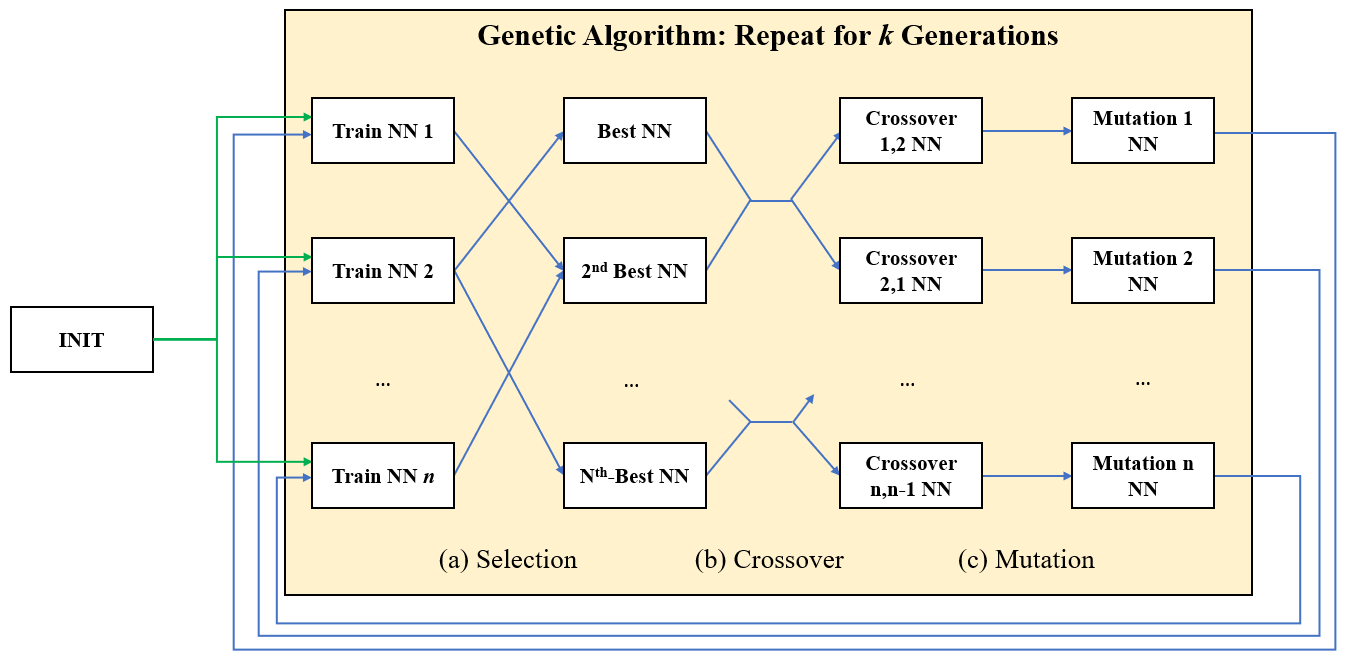
\includegraphics[width=\linewidth]{figures/genetic_overview.PNG}
    \caption{Genetic Algorithm Overview}
    \label{fig:genetic}
\end{figure}

The genetic algorithm is initialized using the baseline traffic light timings generated by the SUMO traffic simulation. This baseline timing is akin to a simple static timed traffic light control scheme which does not consider real-time traffic flow. Using this baseline timing scheme as a starting point, a population size of $n$ neural networks (NN) is trained via the methodology outlined in section ~\ref{NN_subsection}.

For the selection step in the genetic algorithm, we developed a fitness function to compare different neural networks. Currently, the fitness function simply returns the total vehicle travel time from a simulation executed using the given neural network traffic control timings. This is a valid comparison as long as traffic flow is consistent amongst all simulations being compared, which was the case between all neural networks. For a given simulated traffic flow demand, an optimal traffic control timing scheme would cause total vehicle travel time to converge to a nonzero value corresponding to the case where all vehicles traverse the grid without stopping nor slowing down. In practice, this hypothetical minimum would not be possible if traffic flow is high enough such that two vehicles attempt to cross an intersection from different directions simultaneously. Thus, the optimal (i.e. minimum) total vehicle travel time is a function of both city grid layout and traffic flow. In the last step of the selection process, the neural networks are sorted from best to worst according to the total travel time fitness function.

Next, the crossover step in the genetic algorithm is performed by randomly combining the hidden weights of two parent neural networks. Iterating through all weights in the NN, the given weight for the child NN is selected to be equivalent to the corresponding weight for parent $A$ with a probability of 50\%, and similarly the weight is selected to be equivalent to the corresponding weight for parent $B$ with a probability of 50\%.

The mutation step in the genetic algorithm occurs concurrently with the crossover step. The given weight for the child NN is set at random with a probability equivalent to the mutation rate (currently set to 7\%) instead of assigning this weight to be equivalent to a corresponding parent NN weight.

Finally, the genetic algorithm is repeated for $k$ generations. However, for all generations after the initial one (i.e. for all $k > 1$), the initialization step using the baseline traffic light timings is skipped and instead the initial population for generation $i$ is equivalent to the population resulting from the final mutation step of generation $i-1$. After the $k$-th generation of the genetic algorithm, the top performing NN is found using the total travel time fitness function and returned as the final traffic light NN.

\subsection{Traffic Light Neural Network} \label{NN_subsection}

\begin{figure}[htp]
    \centering
    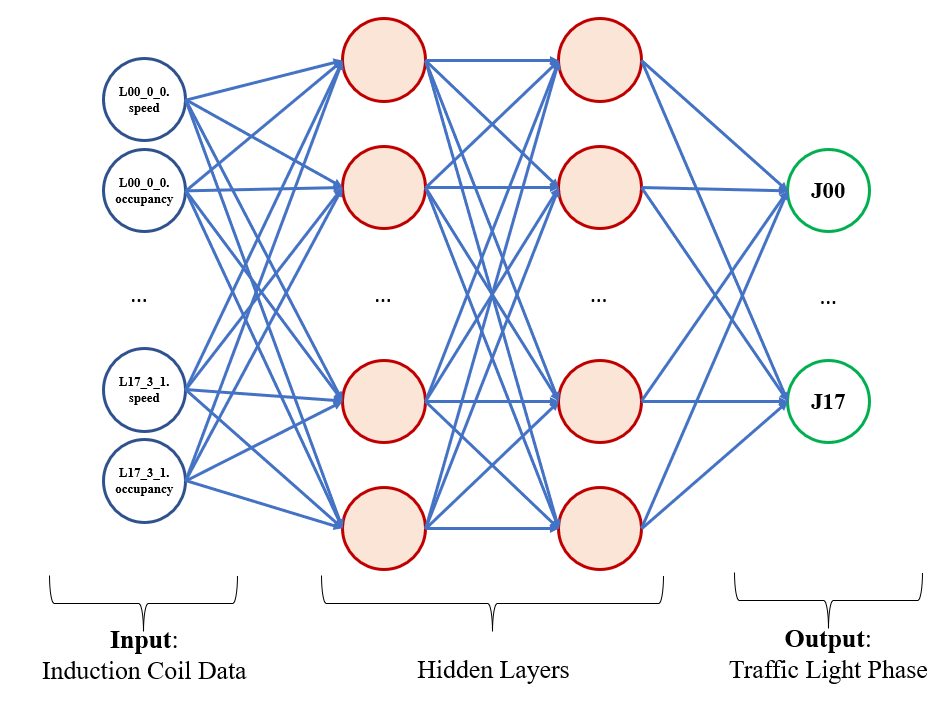
\includegraphics[width=8cm]{figures/NN_overview.PNG}
    \caption{Traffic Light Neural Network}
    \label{fig:nn_overview}
\end{figure}

A traffic agent in our code is defined as a module that, upon each step of the simulation (which represents one second of simulation time) the agent is notified of the step and allowed to query and modify the simulation. Our trained agent is an agent that queries and tracks the phase duration of each light junction. When a phase is over, and switches to the next state in its pattern, a neural network within the agent is queried. The network takes in from each induction loop on the map two variables: the speed in meters per second $(\frac{m}{s})$ of vehicles that passed over the induction loop since the last simulation step, and the occupancy percentage of the induction loop since the last simulation step. These are fed through an adjustable hidden layer(default 100 neurons)  via a reLU function 
\begin{equation} 
    ReLU(x) = (x > 0) * x
\end{equation}
in a fully connected network  layer that is equivalent to the number of junctions on the map (9 for our Chicago example),see Figure ~\ref{fig:nn_overview} and finally output through a sigmoid function (limiting the output values to $(0,1)$)

\begin{equation} 
    S(x) = \frac{1}{1 + e^{-x}}
\end{equation}

This value is mapped to the range of a minimum and maximum allowed time for the transition - currently between 3 and 25 seconds. Each output neuron is mapped to a specific light junction, so this output is assigned to the junction that needs its next timing assignment.

This methodology is applied within an agent we refer to as the "Neural Network Agent". We explored other approaches as well while we tried to find improved performance.

\subsection{Additional Neural Network Agents} \label{NN_subsection}

We attempted to increase the available data handed to the neural network at inference time. To this end, we created two new agents, the "Average Network Agent" and the "History Network Agent". The Average Network agent would take the last $N$ observations of data from our sensors and average them, so that the agents were working on data over a longer time period vs just reacting to a singular point in time when the duration changes. The History Network agent does not average this data, but instead feeds all data over the last $N$ steps to the network without averaging, allow the network itself to decide how to handle data from older time steps. For the purposes of this paper we often utilized $N$ to be either $5$ or $10$.

These agents performed generation mating, mutation, and training exactly the same as their originator the Neural Network Agent.

\subsection{Schedule Agent} \label{NN_subsection}

When we did not reach the desired results, we also created a "Schedule Agent". This agent did not utilize a neural network within, but instead had a preset static schedule for the duration of each phase for ecah traffic light junction. When a light phase changed within the simulation, a duration was referenced within this agent and applied.

The agent would perform similar mating, mutation, and generational changes similar to the neural network agent. Instead of swapping neurons, however, the schedules would swap specific times for specific lights. A triggered mutation would generate a new random time.


\section{Experimental Results \& \\ Discussion}

\subsection{Simulation Environment}

For testing traffic light control algorithms, we opted to use an industry standard, open source traffic simulation environment named SUMO (Simulation of Urban MObility). SUMO is widely used for research into traffic management and congestion, and provides practically all the tools necessary for analysis. SUMO provides the capability to design and test custom street networks, intersection configurations including various types of traffic lights, and create simulated traffic flow.  Through custom Python scripts, control can be exhibited over many of the simulation elements including traffic light parameters.

\begin{figure}[htp]
    \centering
    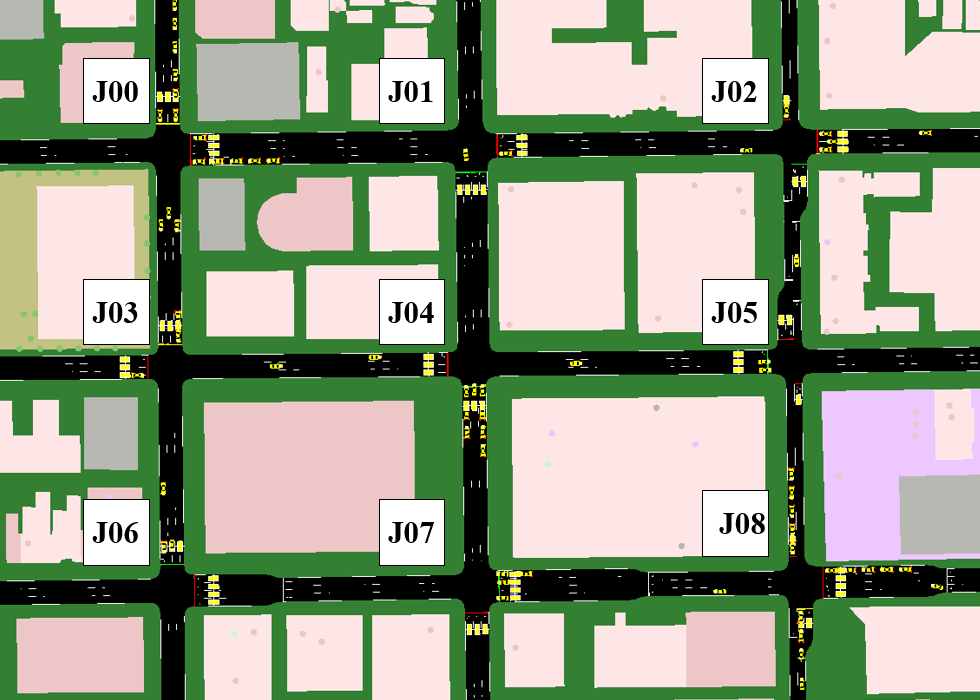
\includegraphics[width=\linewidth]{figures/sumo_chicago2_sim.PNG}
    \caption{SUMO Traffic Simulation Environment}
    \label{fig:sumo_sim}
\end{figure}

SUMO also provides a ready-built tool called OSMWebWizard which allows a user to create a SUMO traffic simulation using real world map data. We utilized OSMWebWizard to create a SUMO traffic scenario comprised of a network of 9 traffic lights arranged in a 3 x 3 grid from the city of Chicago (see Figure ~\ref{fig:sumo_sim}). A subset of the Chicago city grid was chosen because it is designed in a relatively even rectilinear manner aligned approximately North-South and East-West, well suited for a proof of concept environment for this paper.

At each traffic light intersection we added simulated induction loop detectors to each lane incoming to the intersection for the purpose of detecting traffic flow local to a given intersection. The intent is to use these induction loop detectors as a generic means for detecting traffic flow which can then be used as an input for training the traffic light neural network. A fielded application of this project could use actual induction loop detectors or could use a different means for detecting traffic, such as visible spectrum cameras implementing computer vision algorithms to detect the presence and location of vehicles. 

The SUMO environment also includes TraCI - (TRAffic Control Interface) - a python package for communicating with and controlling SUMO's simulation engine.  With this we built our own control interface to streamline control of the simulator with our genetic trainer and traffic light control agents. 

Sumo gives the ability to include realistic compounding elements like pedestrians, crosswalks, bicycles, bike lanes, tram lines, and railroad crossings.  We have omitted these elements at this stage in order to focus of the effects of light control.  Other vehicle types are also available in SUMO such as trucks, delivery vans, busses, EVs and trams.  For a similar reason we have chosen at this time not to include these.  

\subsection{Metrics}

The following metrics were the primary means by which we compared one agent to another:

\begin{itemize}
\item Total Travel Time: the total travel time of all vehicles traversing the simulation
\item Total Depart Delay: the total time vehicles had to wait before starting their journeys
\item Average Vehicle Speed: The average trip speed of a vehicle through the simulation
\end{itemize}

Both Total Travel Time and Average Vehicle Speed were evaluated for usage as the fitness function for our genetic algorithm, see section ~\ref{Fitness_Func_subsection} for further discussion.

\subsection{Comparisons}

SUMO default traffic lights are set for 90 second cycles evenly split by direction.  Here, we will use this as a proxy for scheduled lights which are common in cities and as a baseline for comparison for our other models.  We also plan to compare a randomly generated schedule of phases and durations.


By default, the SUMO simulation generated from Chicago city data uses a simple timing schedule defined in Table ~\ref{tab:baseline_params} regardless of real-time traffic flow. At the conclusion of the last phase (P3 or P5 depending on traffic light), the cycle resets to P0.

\subsection{Null Agent}

The null agent was the baseline for comparison for all other agents. This agent utilizes the SUMO default traffic light phase timings described in Table ~\ref{tab:baseline_params}. Most likely the SUMO default traffic light timings are set by similar heuristics as set forth in (\cite{USDOT}), wherein the traffic light phase durations are set to clear the queue of vehicles waiting at the light for a given cycle with a high degree of confidence.

\begin{table}[H]
    \centering
    \begin{tabular}{|c|c|c|c|c|c|c|}
        \hline
         Traffic Light & P0 & P1 &  P2 & P3 & P4 &  P5 \\
        \hline\hline
        J00 & 39 &	6 & 39 & 6 & - & - \\
        \hline
        J01 & 39 &	6 & 39 & 6 & - & - \\
        \hline
        J02 & 33 &	6 & 6 & 6 & 33 & 6 \\
        \hline
        J03 & 39 &	6 & 39 & 6 & - & - \\
        \hline
        J04 & 39 &	6 & 39 & 6 & - & - \\
        \hline
        J05 & 33 &	6 & 6 & 6 & 33 & 6 \\
        \hline
        J06 & 39 &	6 & 39 & 6 & - & - \\
        \hline
        J07 & 39 &	6 & 39 & 6 & - & - \\
        \hline
        J08 & 33 &	6 & 6 & 6 & 33 & 6 \\
        \hline
    \end{tabular}
    \caption{Null Agent Phase Durations (sec)}
    \label{tab:baseline_params}
\end{table}

Summary results for the null agent are presented in Table ~\ref{tab:null_agent_perf}. The null agent was ultimately found to have the lowest demonstrated total travel time and total departure delay, and highest average vehicle speed.

\begin{table}[H]
    \centering
    \begin{tabular}{|c|c|c|c|c|c|c|}
        \hline
         Metric & Value & Units \\
        \hline\hline
        Total Travel Time & 209,994 & $sec$ \\
        \hline
        Total Depart Delay & 1616 & $sec$ \\
        \hline
        Average Vehicle Speed & 9.18 & $m/s$ \\
        \hline
    \end{tabular}
    \caption{Null Agent Performance}
    \label{tab:null_agent_perf}
\end{table}

\subsection{Random Agent}

The random agent will, upon expiration of a light phase's duration, then select a random time duration (between $3$ and $20$ seconds) for the next phase. This agent was created to demonstrate a baseline environmental response to terrible management planning.

\begin{table}[H]
    \centering
    \begin{tabular}{|c|c|c|c|c|c|c|}
        \hline
         Metric & Value & Units \\
        \hline\hline
        Total Travel Time & 520,882 & $sec$ \\
        \hline
        Total Depart Delay & 7158 & $sec$ \\
        \hline
        Average Vehicle Speed & 4.96 & $m/s$ \\
        \hline
    \end{tabular}
    \caption{Random Agent Performance}
    \label{tab:random_agent_perf}
\end{table}

\subsection{Neural Network Agent}

The neural network agent, our first attempt at an agent, controlled lights by generating a new light duration for each junction as it switched its phase. The network would dynamically change these scheduled times as the simulation ran.

\begin{table}[H]
    \centering
    \begin{tabular}{|c|c|c|c|c|c|c|}
        \hline
         Metric & Value & Units \\
        \hline\hline
        Total Travel Time & 389,471 & $sec$ \\
        \hline
        Total Depart Delay & 5193 & $sec$ \\
        \hline
        Average Vehicle Speed & 7.61 & $m/s$ \\
        \hline
    \end{tabular}
    \caption{Neural Network Agent Performance}
    \label{tab:nn_agent_perf}
\end{table}

\subsection{Average Network Agent}

The Average Network Agent would take $N$ of the past time steps (in this case, $5$), and average data from this to input into the neural network. This was done to provide a more robust look into traffic performance as the network inferred possible timing durations.

\begin{table}[H]
    \centering
    \begin{tabular}{|c|c|c|c|c|c|c|}
        \hline
         Metric & Value & Units \\
        \hline\hline
        Total Travel Time & 402,713 & $sec$ \\
        \hline
        Total Depart Delay & 5827 & $sec$ \\
        \hline
        Average Vehicle Speed & 6.67 & $m/s$ \\
        \hline
    \end{tabular}
    \caption{Average Network Agent Performance}
    \label{tab:average_agent_perf}
\end{table}

\subsection{History Network Agent}

The History Network Agent would feed the last $N$ steps ($5$ in this case) of data into the network, allowing the network to decide what data was relevant to it. It did perform slightly better than the Average Network Agent.

\begin{table}[H]
    \centering
    \begin{tabular}{|c|c|c|c|c|c|c|}
        \hline
         Metric & Value & Units \\
        \hline\hline
        Total Travel Time & 398,615 & $sec$ \\
        \hline
        Total Depart Delay & 5578 & $sec$ \\
        \hline
        Average Vehicle Speed & 6.82 & $m/s$ \\
        \hline
    \end{tabular}
    \caption{History Network Agent Performance}
    \label{tab:history_agent_perf}
\end{table}

\subsection{Schedule Agent}

The schedule agent had a static duration schedule for each phase of each light junction. This schedule was generated as a part of the agent itself and evolved over time. This approach was a departure of other designed agents within this paper, provided as more of a baseline test to see if static schedules, especially ones that were designed by another agent, were inherently better than dynamic scheduling agents.

\begin{table}[H]
    \centering
    \begin{tabular}{|c|c|c|c|c|c|c|}
        \hline
         Metric & Value & Units \\
        \hline\hline
        Total Travel Time & 402,572 & $sec$ \\
        \hline
        Total Depart Delay & 6181 & $sec$ \\
        \hline
        Average Vehicle Speed & 5.92 & $m/s$ \\
        \hline
    \end{tabular}
    \caption{Schedule Agent Performance}
    \label{tab:scheduled_agent_perf}
\end{table}

\subsection{Incremental Agent}

The incremental agent used the same structure and logic as the neural network agent, except for the key difference in what specific output the agent had control over. The output of the neural network agent was the phase duration for all traffic lights; in contrast, the output of the incremental agent was the decision of whether to increment the traffic light phase for any or all of the traffic lights. The rationale of this modification is that incrementing traffic light phase is a more immediate, direct form of control compared with adjusting the duration of the subsequent traffic light phase. Importantly, the incremental agent also enforced a minimum phase duration of 3 seconds. It was thought that any phase durations less than 3 seconds would be unrealistically quick for a human driver to react to.

\begin{figure}[htp]
    \centering
    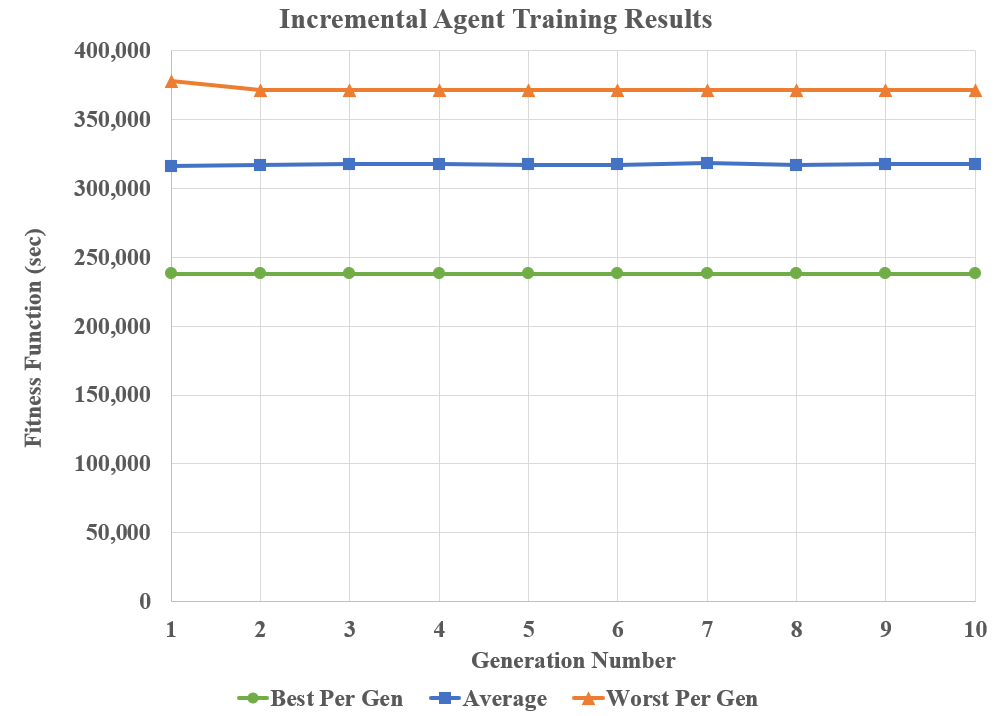
\includegraphics[width=\linewidth]{figures/inc_agent_training.PNG}
    \caption{Training Results for Incremental Agent}
    \label{fig:inc_agent_training}
\end{figure}

Other than the method by which the agent attempted to control the traffic lights, the incremental agent was implemented identically to the neural network agent, including the same genetic algorithm for selection, crossover, and mutation of the best individuals of a given generation. Figure ~\ref{fig:inc_agent_training} presents a graph of best, worst, and average fitness (aka total travel time) as a function of generation number for the incremental agent. This graph shows that there was no improvement or any significant change in measured fitness over the course of 10 generations.

A similar result was found for the schedule agent and neural network agent, namely no discernible change over a relatively small number of generations. See Section ~\ref{conclusion_section} for a detailed discussion of the possible reasons why our genetic algorithm did not produce a significant improvement in fitness over our training period.

Summary performance metrics for the best individual incremental agent after 10 generations of evolution are shown in Table ~\ref{tab:inc_agent_perf}. The incremental agent demonstrated slightly higher total travel time and total departure delay and lower average vehicle speed compared with the null agent, though it outperformed the neural network, schedule, and random agents.

\begin{table}[H]
    \centering
    \begin{tabular}{|c|c|c|c|c|c|c|}
        \hline
         Metric & Value & Units \\
        \hline\hline
        Total Travel Time & 238,269 & $sec$ \\
        \hline
        Total Depart Delay & 1797 & $sec$ \\
        \hline
        Average Vehicle Speed & 8.46 & $m/s$ \\
        \hline
    \end{tabular}
    \caption{Incremental Agent Performance}
    \label{tab:inc_agent_perf}
\end{table}

\subsection{Exploring Different Fitness function} \label{Fitness_Func_subsection}
To explore sensitivity to number of vehicles in the network, we examined altering the fitness function from total travel time to average speed.  We found results did not converge quickly and did not exceed the performance of our baseline.
\begin{table}[H]
    \centering
    \begin{tabular}{|c|c|c|c|c|c|c|}
        \hline
         Metric & Value & Units \\
        \hline\hline
        Total Travel Time & 432,102 & $sec$ \\
        \hline
        Route Length & 632.11 & $m$ \\
        \hline
        Average Vehicle Speed & 5.26 & $m/s$ \\
        \hline
    \end{tabular}
    \caption{Speed Fitness Performance}
    \label{tab:speed_results}
\end{table}


The performance of the neural network agent using average vehicle speed as the fitness function (instead of total travel time) is shown in Table ~\ref{tab:speed_results}. The performance of the neural network agent did not noticeably improve using this different fitness function.

\subsection{Summary Agent Comparison}

See Figure ~\ref{fig:agent_comparison} for a comparison of the best individual of each agent type as determined by minimum fitness function (total travel time). 

\begin{figure}[htp]
    \centering
    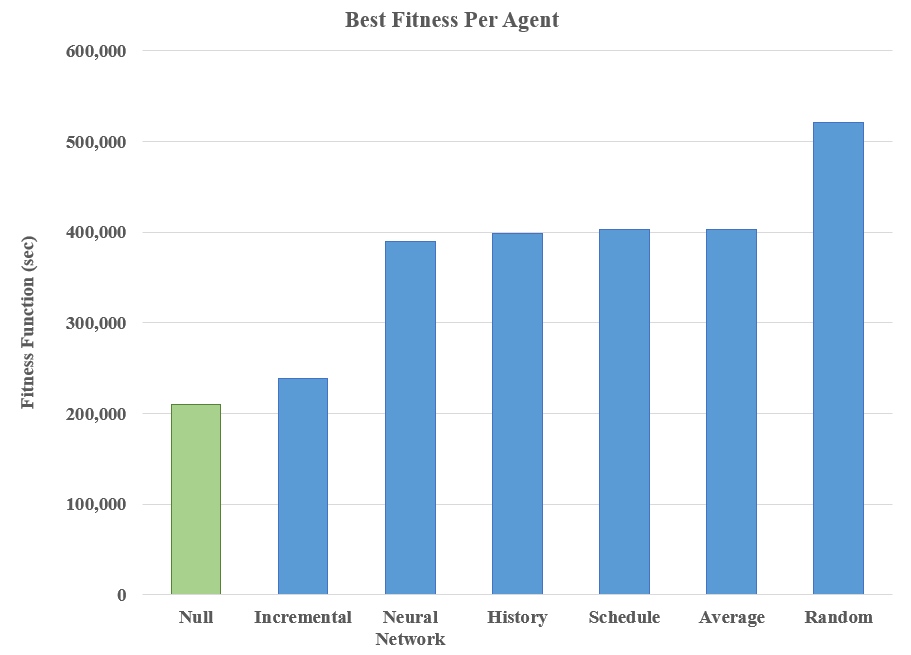
\includegraphics[width=\linewidth]{figures/agent_summary.PNG}
    \caption{Agents Compared by Best Fitness}
    \label{fig:agent_comparison}
\end{figure}

Overall we found that the null agent demonstrated the lowest total travel time (our principle metric of comparison) in addition to lowest total departure delay and fastest average vehicle speed. The incremental agent with a minimum phase time of 3 seconds was somewhat worse at about 240,000 seconds, while the neural network agent and schedule agent each had a total travel time of approximately 400,000 seconds.

The worst agent was the random agent, with total travel time over 500,000 seconds


\section{Conclusions} \label{conclusion_section}
We attempted to modify multiple aspects of our genetic algorithm in order to minimize total travel time in our simulation. In addition to defining our fitness function as equivalent to total vehicle travel time, we also ran some simulations using average vehicle speed as our fitness function. We tested two different sizes of a city grid, both 3x3 and 3x6. Lastly as outlined earlier in the presentation, we tested different agent implementations.

Despite our best efforts we were ultimately unable to demonstrate a significant improvement in measured fitness over the course of 10-20 generations. One possible reason is that our genetic algorithm only attempted to update agent weights once per generation, and given the complexity of the problem perhaps this is far too few generations. The input layer to our neural network was a vector of 108 elements, the hidden layers had hundreds of neurons, and the output layer attempted to set 9 different traffic light phases so its possible 10-20 total updates of weights is far too few.

However, we were also severely constrained in the number of generations we could simulate due to time constraints. Running only 10 generations with a population size of 10 per generation would take approximately 10 hours of real computing time, making it infeasible to test larger numbers of generations in the limited time and computing power allotted for the project.

Finally, it’s possible that the input data we were feeding the neural network was inadequate. We used induction loop occupancy and speed data on each traffic light input lane as input data, where the neural network did not have any predetermined knowledge of the mapping between which induction loops corresponded to which intersections.

As a result of these limitations, none of our agents were able to outperform the default null agent.



\section{Future Work}
As future work, we would attempt to train over many more generations (possibly in the range of 100s of generations) versus the 10-20 we were able to test in this project. This would require much more time or access to faster computing power.

We would also explore making a structural update to the algorithm to attempt to update neural network weights much more often than once per generation. This would help alleviate the simulation bottleneck by allowing the network to learn more quickly.

Lastly, improved vehicle data fed into the neural network would likely improve its ability to learn.


\section{Source Code}
The source code for this project can be found at the following git repository: \url{https://github.com/hlfshell/cs534-project} 


\bibliographystyle{apacite}
\bibliography{references}

\end{document}
